\documentclass{article}
\usepackage{verbatim}
\usepackage{pgfplots}
\pgfplotsset{
  compat=1.14,
}
\usepackage{tikz}
\usepackage{tikzscale}
\usetikzlibrary{external}
\tikzexternalize

\newcommand{\detailtexcount}[1]{%
  \immediate\write18{texcount -merge -sum -incbib -dir #1.tex > #1.wcdetail }%
  \verbatiminput{#1.wcdetail}%
}
 
\newcommand{\quickwordcount}[1]{%
  \immediate\write18{texcount -1 -sum -merge #1.tex > #1-words.sum }%
  \input{#1-words.sum} words%
}
 
\newcommand{\quickcharcount}[1]{%
  \immediate\write18{texcount -1 -sum -merge -char #1.tex > #1-chars.sum }%
  \input{#1-chars.sum} characters (not including spaces)%
}

\begin{document}

%TC:ignore
\quickwordcount{thesis}
\quickcharcount{thesis}
\detailtexcount{thesis}
%TC:endignore
% \resizebox{<horizontal size>}{<vertical size>}{%
%\begin{figure}[h]
%    \caption{TODO}
%    \label{class-distribution}
%    \centering
%    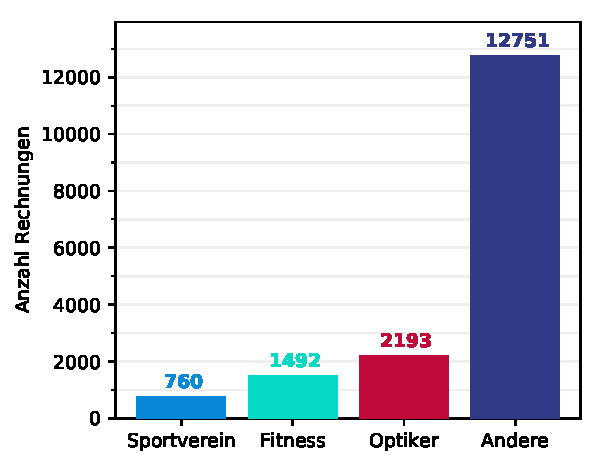
\includegraphics[width=\textwidth, height=100]{graphics/class-weight}
%\end{figure}

\end{document}}